\chapter{Desenvolvimento}
\label{cap:Desenvolvimento}
Nesse capítulo serão abordadas todas as etapas, tal como as técnicas utilizadas para atingir o objetivo de compor um dicionário de léxicos da língua portuguesa específico para detecção de discursos de ódio. Ao final também serão apresentados os resultados esperados com o desenvolvimento, estimando a eficiência e os avanços da pesquisa realizada. 

\section{Geração de \textit{corpus} para Detectar \textit{Haters}}
Como parte fundamental da pesquisa, será criado um dicionário com as palavras mais utilizadas pelos usuários denominados \textit{haters} que pregam discursos de ódio contra indivíduos nas redes sociais.Para a geração do \textit{corpus} desejado serão necessárias algumas etapas de desenvolvimento conforme Figura \ref{fig:fluxodesenvolvimento}. A seguir serão explicadas cada uma das etapas a serem realizadas para a obtenção do dicionário.

\begin{figure}[!h]
\centering 
\caption{Fluxo de atividades para obtenção de \textit{corpus} desejado}
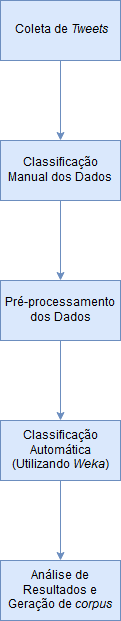
\includegraphics[scale=0.5]{imagens/fluxodesenvolvimento.png}
\legend{Fonte: O Autor}
\label{fig:fluxodesenvolvimento}
\end{figure}

\subsection{Coleta de \textit{Tweets}}
A rede social selecionada para a construção da base de dados será o \textbf{Twitter}, rede social categorizada como \textit{microblogging} em que os usuários realizam atualizações constantes de conteúdo. Para realizar a coleta de dados primeiramente é necessário criar uma conta dentro da \textit{Twitter Developer Platform}\footnote{https://developer.twitter.com/}. Após cadastro a plataforma disponibilizará os \textit{tokens} que serão necessários para a construção do programa de leitura de \textit{tweets} (Figura \ref{fig:twitterdeveloperplatform}).

\begin{figure}[!h]
\centering 
\caption{Tela com \textit{Tokens} Utilizados na \textit{API} do \textit{Twitter}}
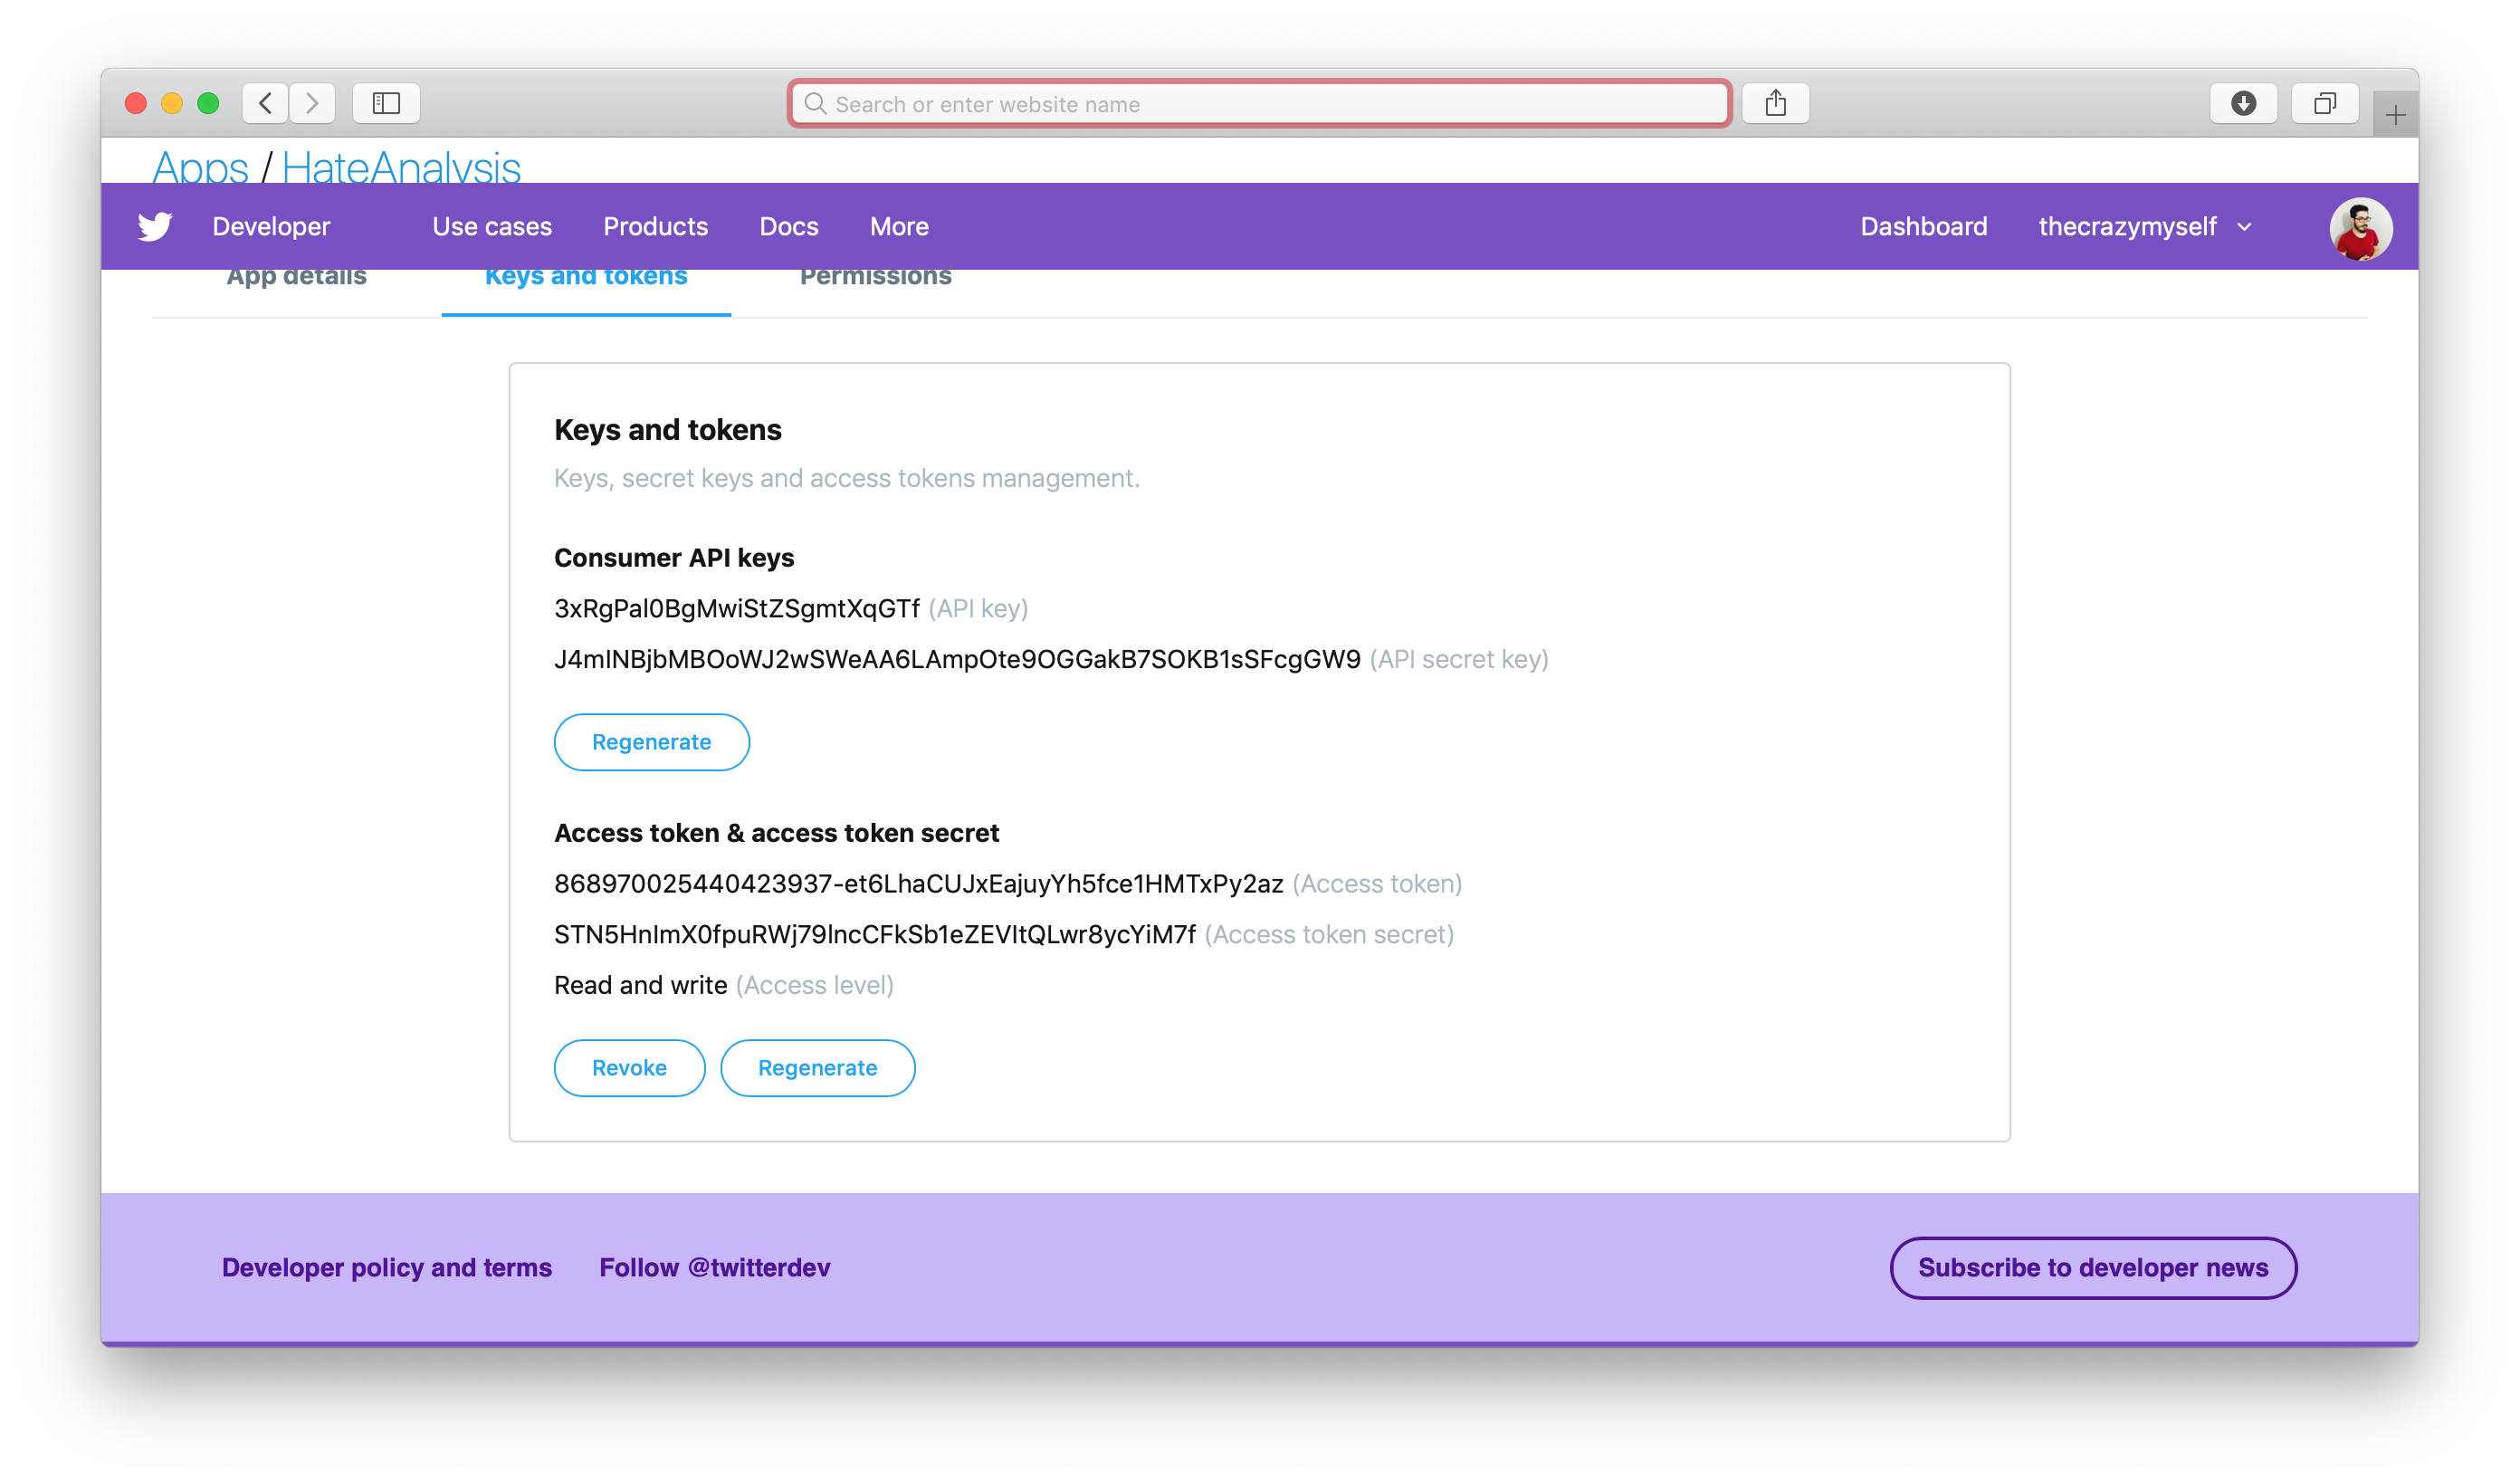
\includegraphics[scale=0.3]{imagens/twitterdeveloperplatform.png}
\legend{Fonte: Twitter Inc.}
\label{fig:twitterdeveloperplatform}
\end{figure}

A linguagem de programação a ser utilizada para a coleta dos dados é a \textit{Java}, linguagem orientada a objetos e multiplataforma mantida pela \textit{Oracle} que é de fácil implementação e bastante utilizada na comunidade \textit{open source} que mantém vários fóruns, \textit{frameworks} e \textit{APIs} constantemente atualizados pela comunidade. A \textit{API} que utilizada será a \textit{Twitter4J}, uma biblioteca não-oficial que permite o acesso aos dados do \textit{Twitter} utilizando a linguagem de programação \textit{Java}, a mesma que será utilizada para a coleta de dados, facilitando o aprendizado da ferramenta bem como a manutenção, se necessário. A \textit{Twitter4J} utiliza autenticação \textit{OAuth}, fazendo uso dos \textit{tokens} disponibilizados pelo \textit{Twitter Developer Platform} e não necessitando de autenticação com e-mail (ou nome de usuário, ) e senha a cada acesso realizado. 

Após a construção do programa de coleta de \textit{tweets}, o próximo passo será encontrar filtros de consulta que irão auxiliar na busca por conteúdos úteis para a geração do \textit{corpus}. O primeiro critério de seleção será a busca por perfis de \textit{influencers} digitais, pessoas cujo ... 

\section{Integração com \textit{Software} Existente}
\section{Resultados Esperados}
\section{Conclusões}
